\NeedsTeXFormat{LaTeX2e}
\documentclass[a4paper, 11pt]{article}

\textheight26.5cm
\topmargin-2cm
\evensidemargin-1.3cm
\oddsidemargin-1.3cm
\textwidth 18.5cm

\usepackage{graphicx}
\usepackage{color}
\usepackage{subcaption}


\begin{document}

\noindent {\large{\bf Tracker + Calorimeter Muon Identification}}

The tracker stations, located in front of calorimeters 13 and 19, provide additional information which can be used to identify and study lost muons.

Particle tracks reconstructed in the two tracking station are extrapolated to the face of calorimeters 13 and 19 respectively (actually 0.6mm in front of each face), where they can be matched to a cluster reconstructed in that calorimeter. To do this, some basic quality, matching, and muon identification criteria are applied, see also see Fig.~\ref{fig:muon_cuts}:

\begin{itemize}
\item track p-value $> 0.05$; 
\item time matching:
  \begin{itemize}
  \item-8~ns $< t_{cluster} - t_{track} < 3 $~ns in Station 13,
    \item-9~ns $< t_{cluster} - t_{track} < 1 $~ns in Station 19;
\end{itemize}
      
\item position matching: $\Delta R = \sqrt{\Delta x_{track-cluster}^2 + \Delta y_{track-cluster}^2} < 30$~mm;
\item muon identification: $-3.2 < log(E/p) < -2.4$;
\item muon identification: $p > 2200$~MeV in Station 13, $p>2350$~MeV in Station 19;
\item muon identification: number of crystals in cluster $\le2$.
%\item muon identifiaction: number of crystals in matched cluster $==1$.
\end{itemize}


\begin{figure}[h]
\centering
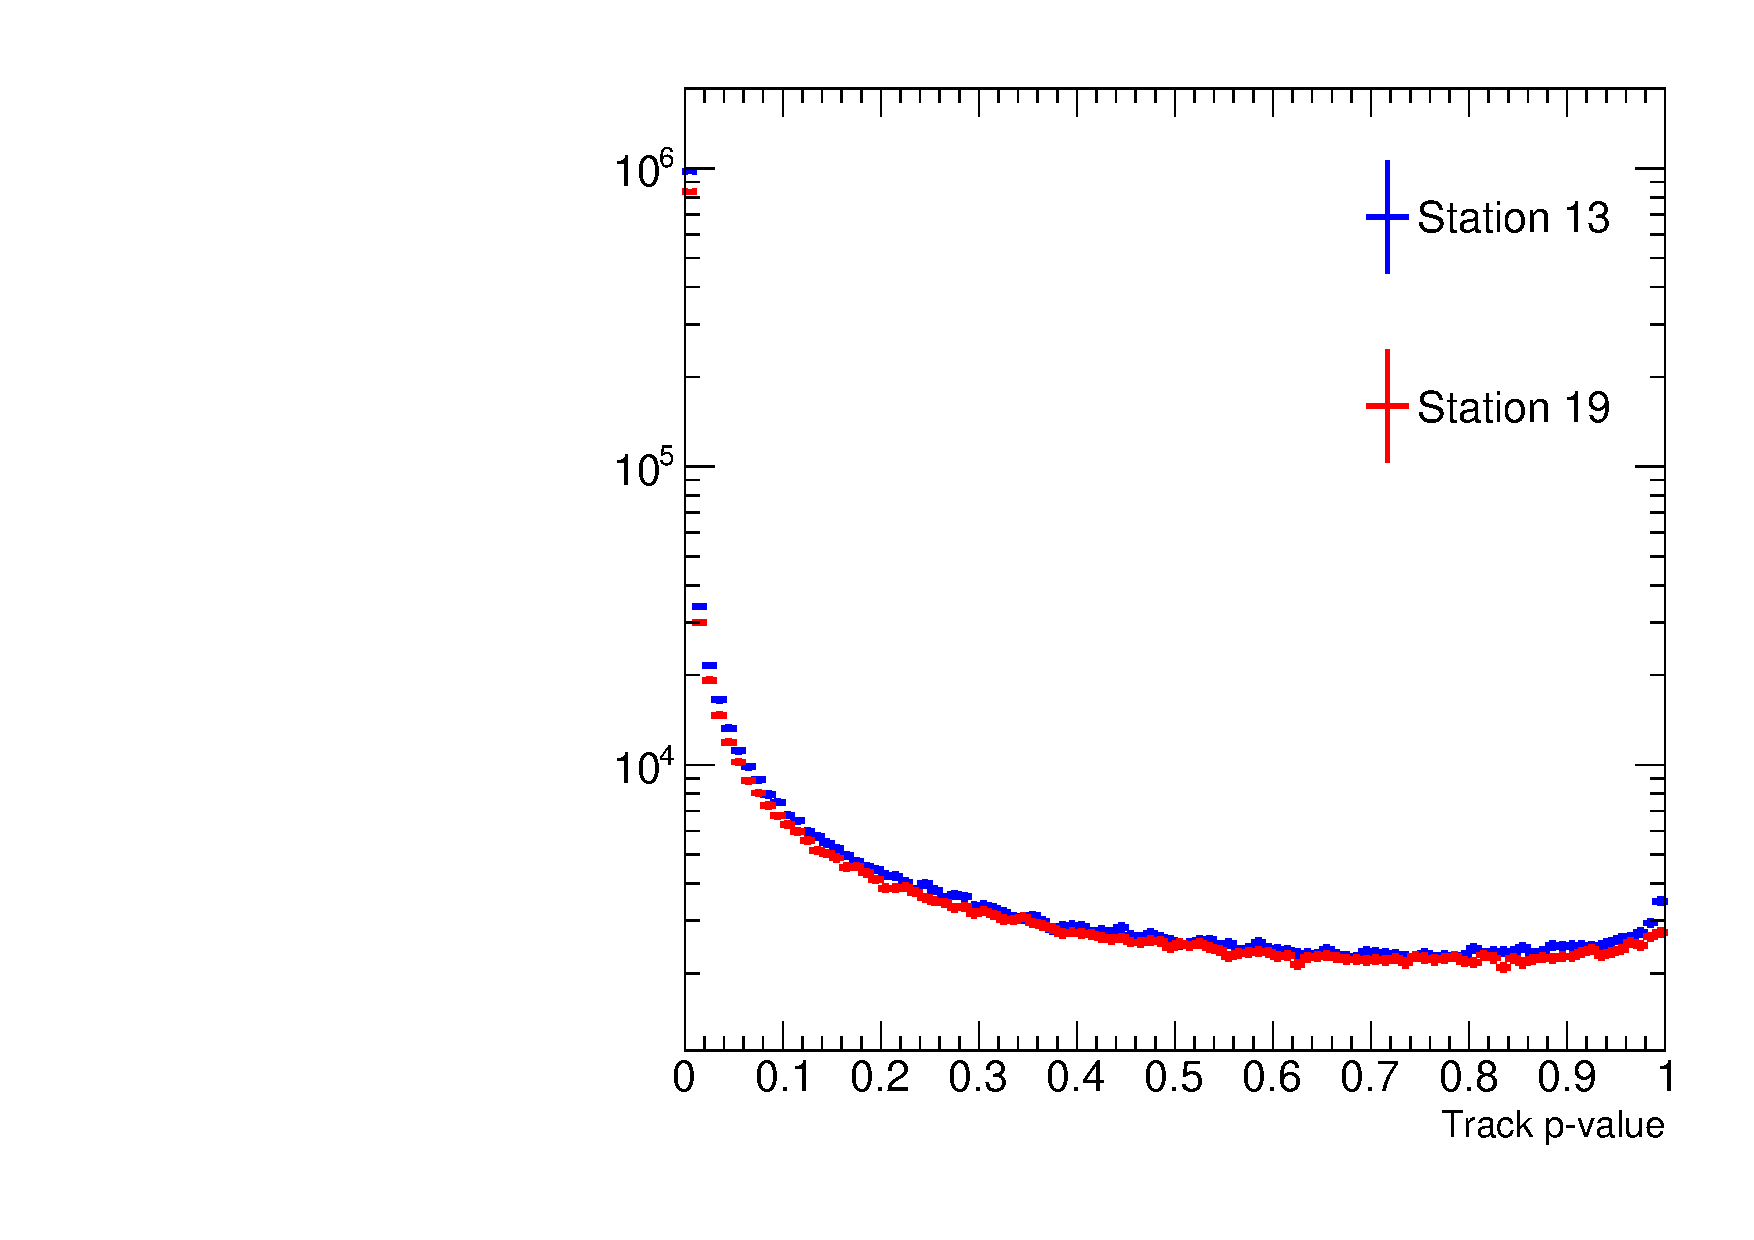
\includegraphics[width=0.18\textwidth]{figures/St13_qc_pval.pdf}
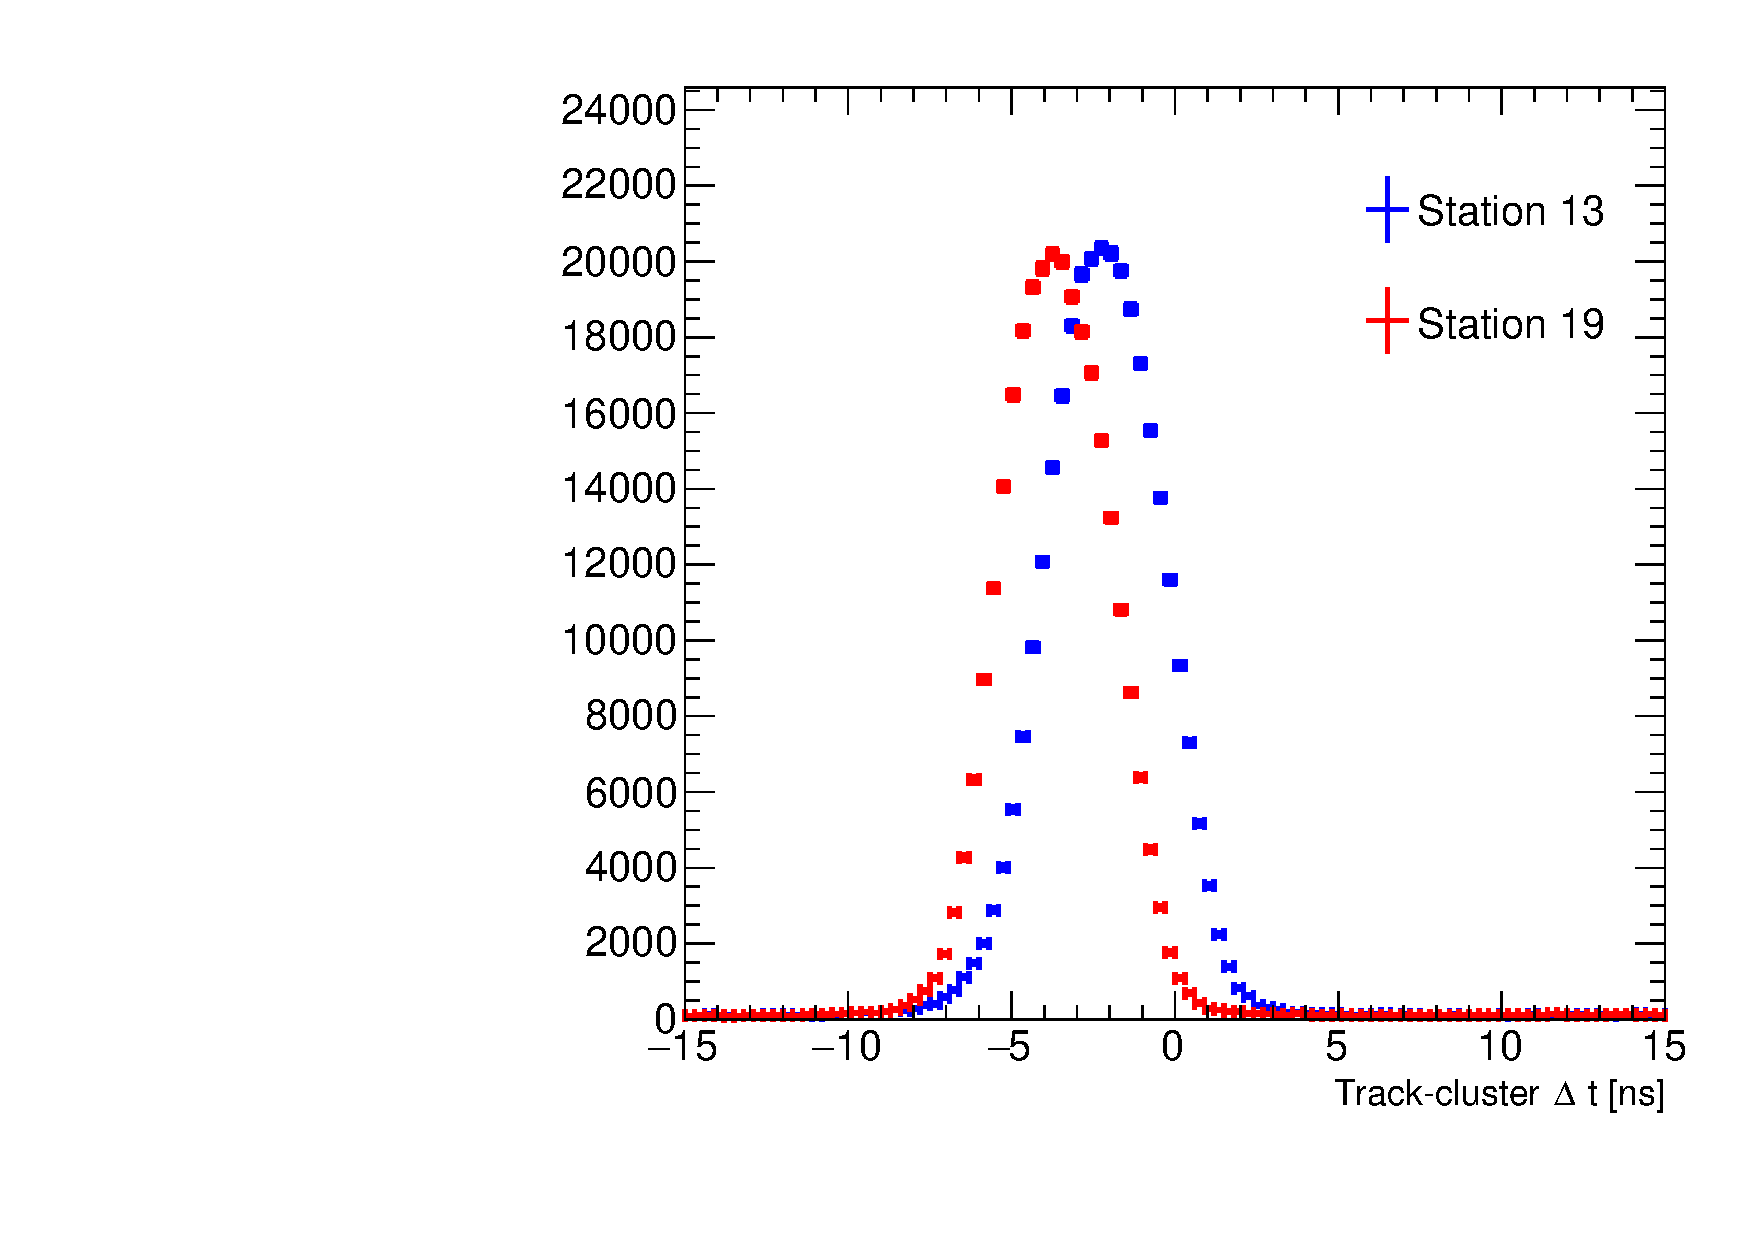
\includegraphics[width=0.18\textwidth]{figures/St13_qc_dt.pdf}
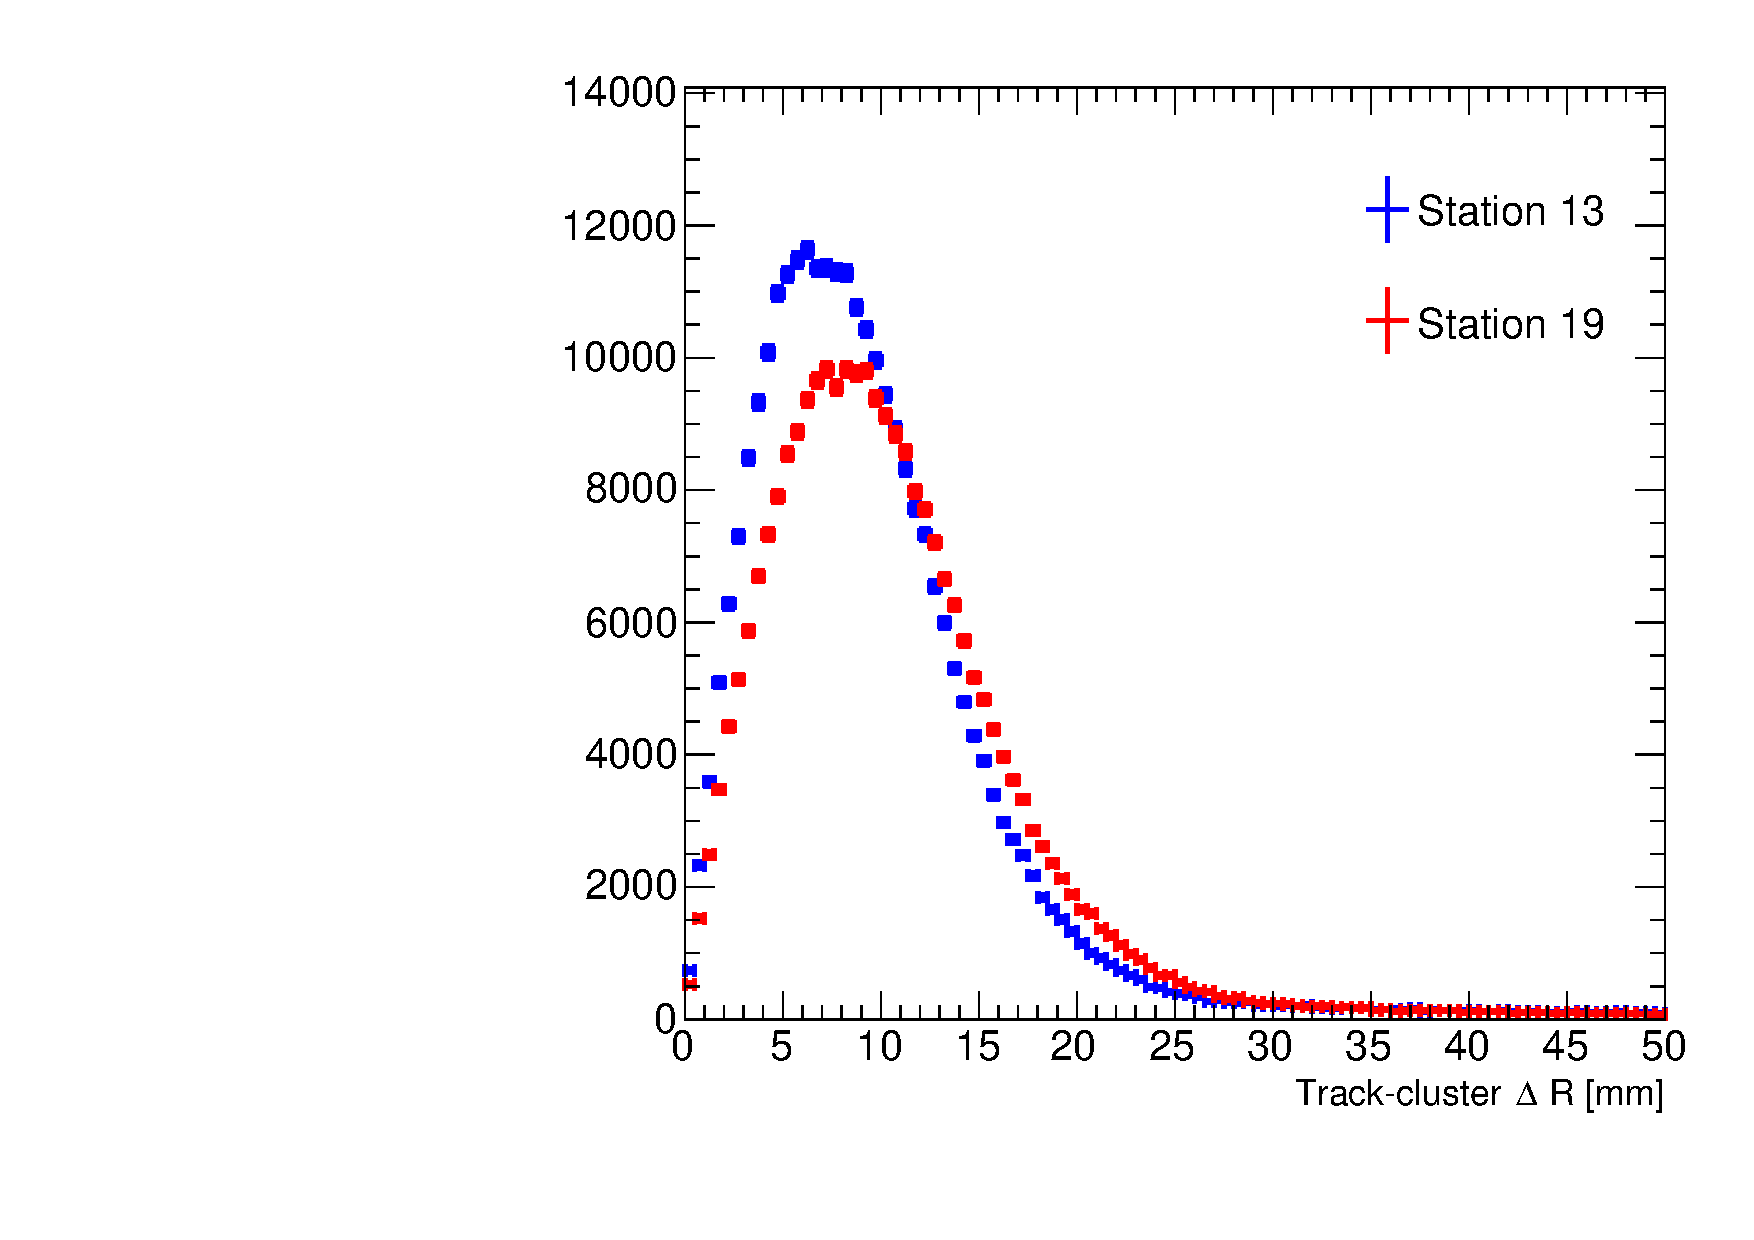
\includegraphics[width=0.18\textwidth]{figures/St13_qc_dR.pdf}
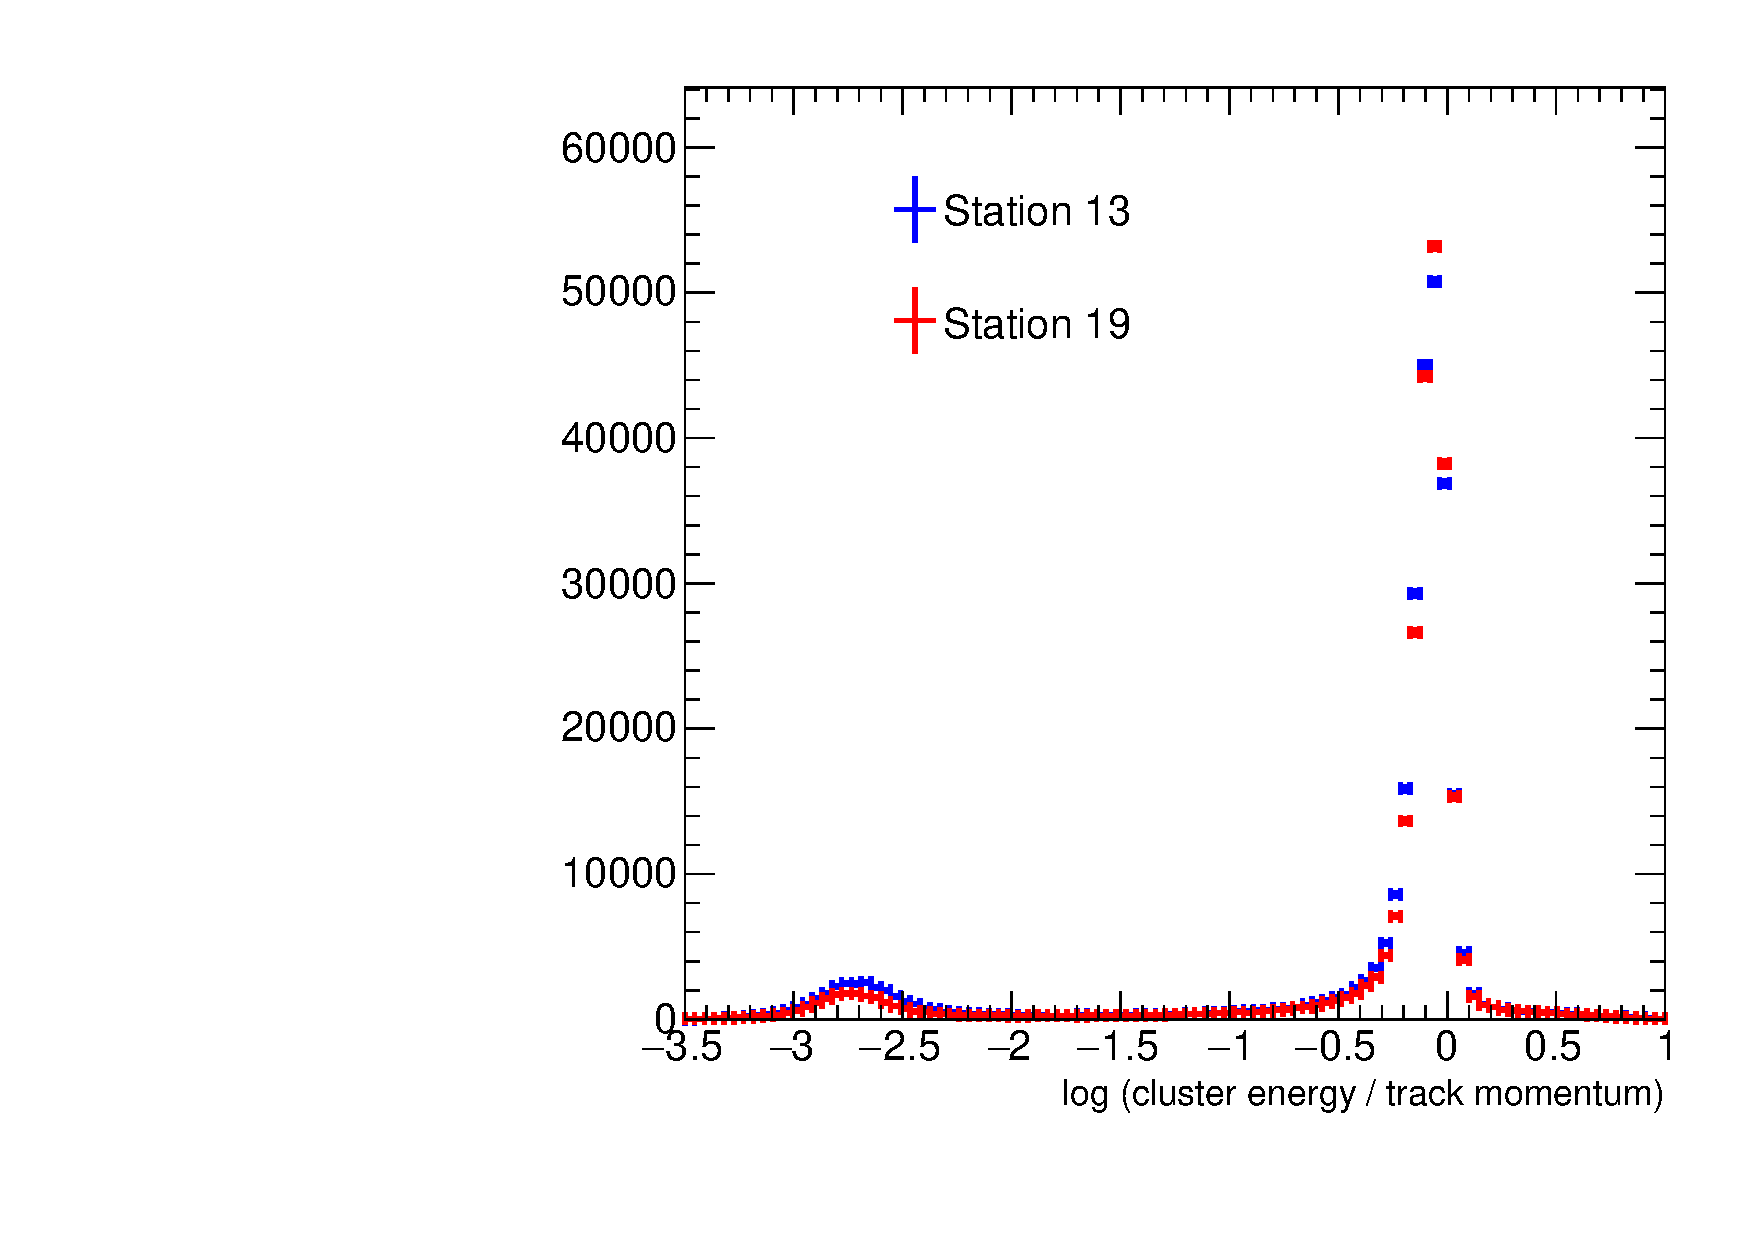
\includegraphics[width=0.18\textwidth]{figures/St13_qc_Eop.pdf}
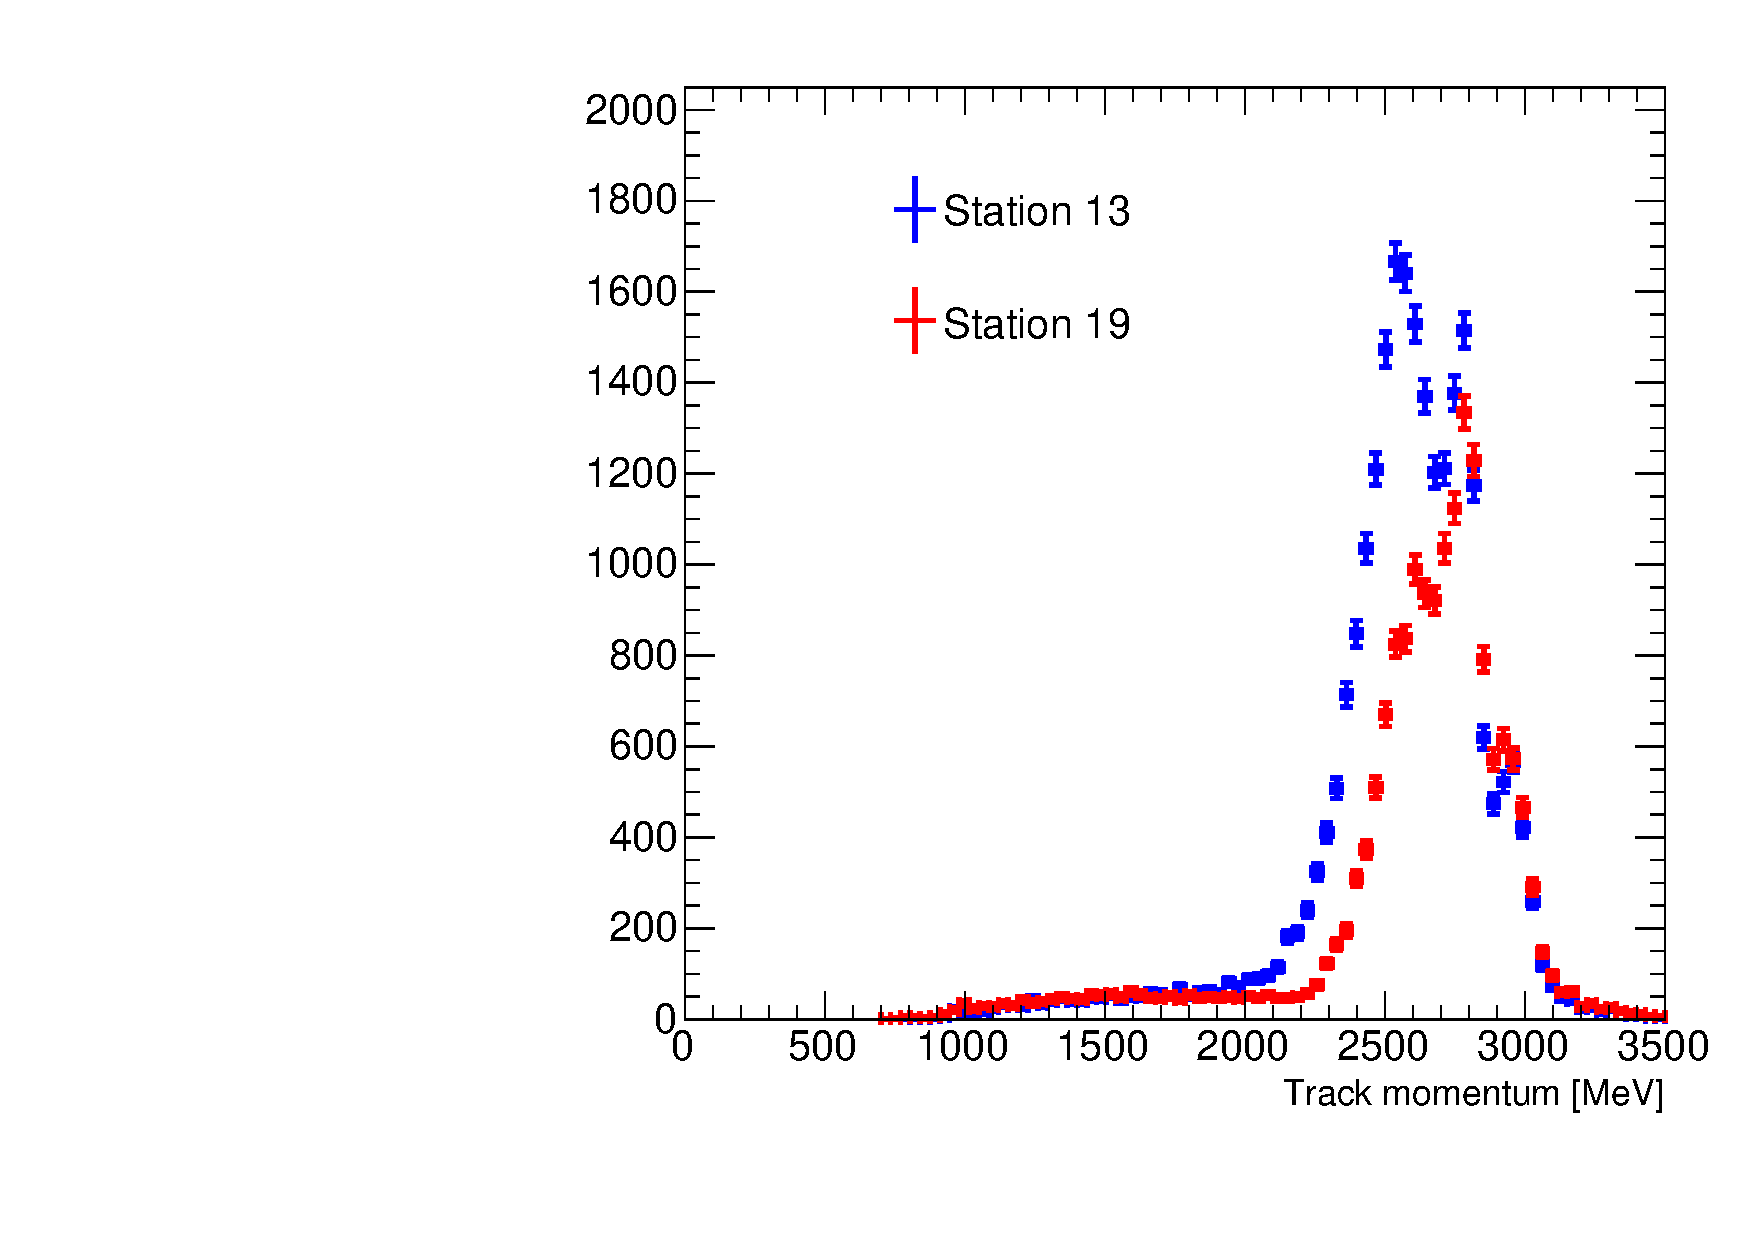
\includegraphics[width=0.18\textwidth]{figures/St13_qc_p.pdf}
\caption{Muon selection based on the tracker + calorimeter. Left: the track p-value distribution; second left: the time difference between tracker and calorimeter; middle: the $\Delta R$ matching between track and calorimeter cluster; second right: the $log(E/p)$ distribution for track and matched cluster, right: the track momentum distribution. Distributions are shown after selecting based on all previous distributions. \label{fig:muon_cuts}}
\end{figure}


It can be seen that there are small differences in the muon populations between Station 13 and Station 19. Specifically, a small shift in the timing inter-calibration between tracker and calorimeter; the spacial matching between tracker and calorimeter; and a different momentum distribution. The low momentum tail after applying all other cuts is found to be positrons hitting the edge of the calorimeters and therefore only depositing a small fraction of their energy (and hence passing the E/p cut).




\begin{figure}[h]
\centering
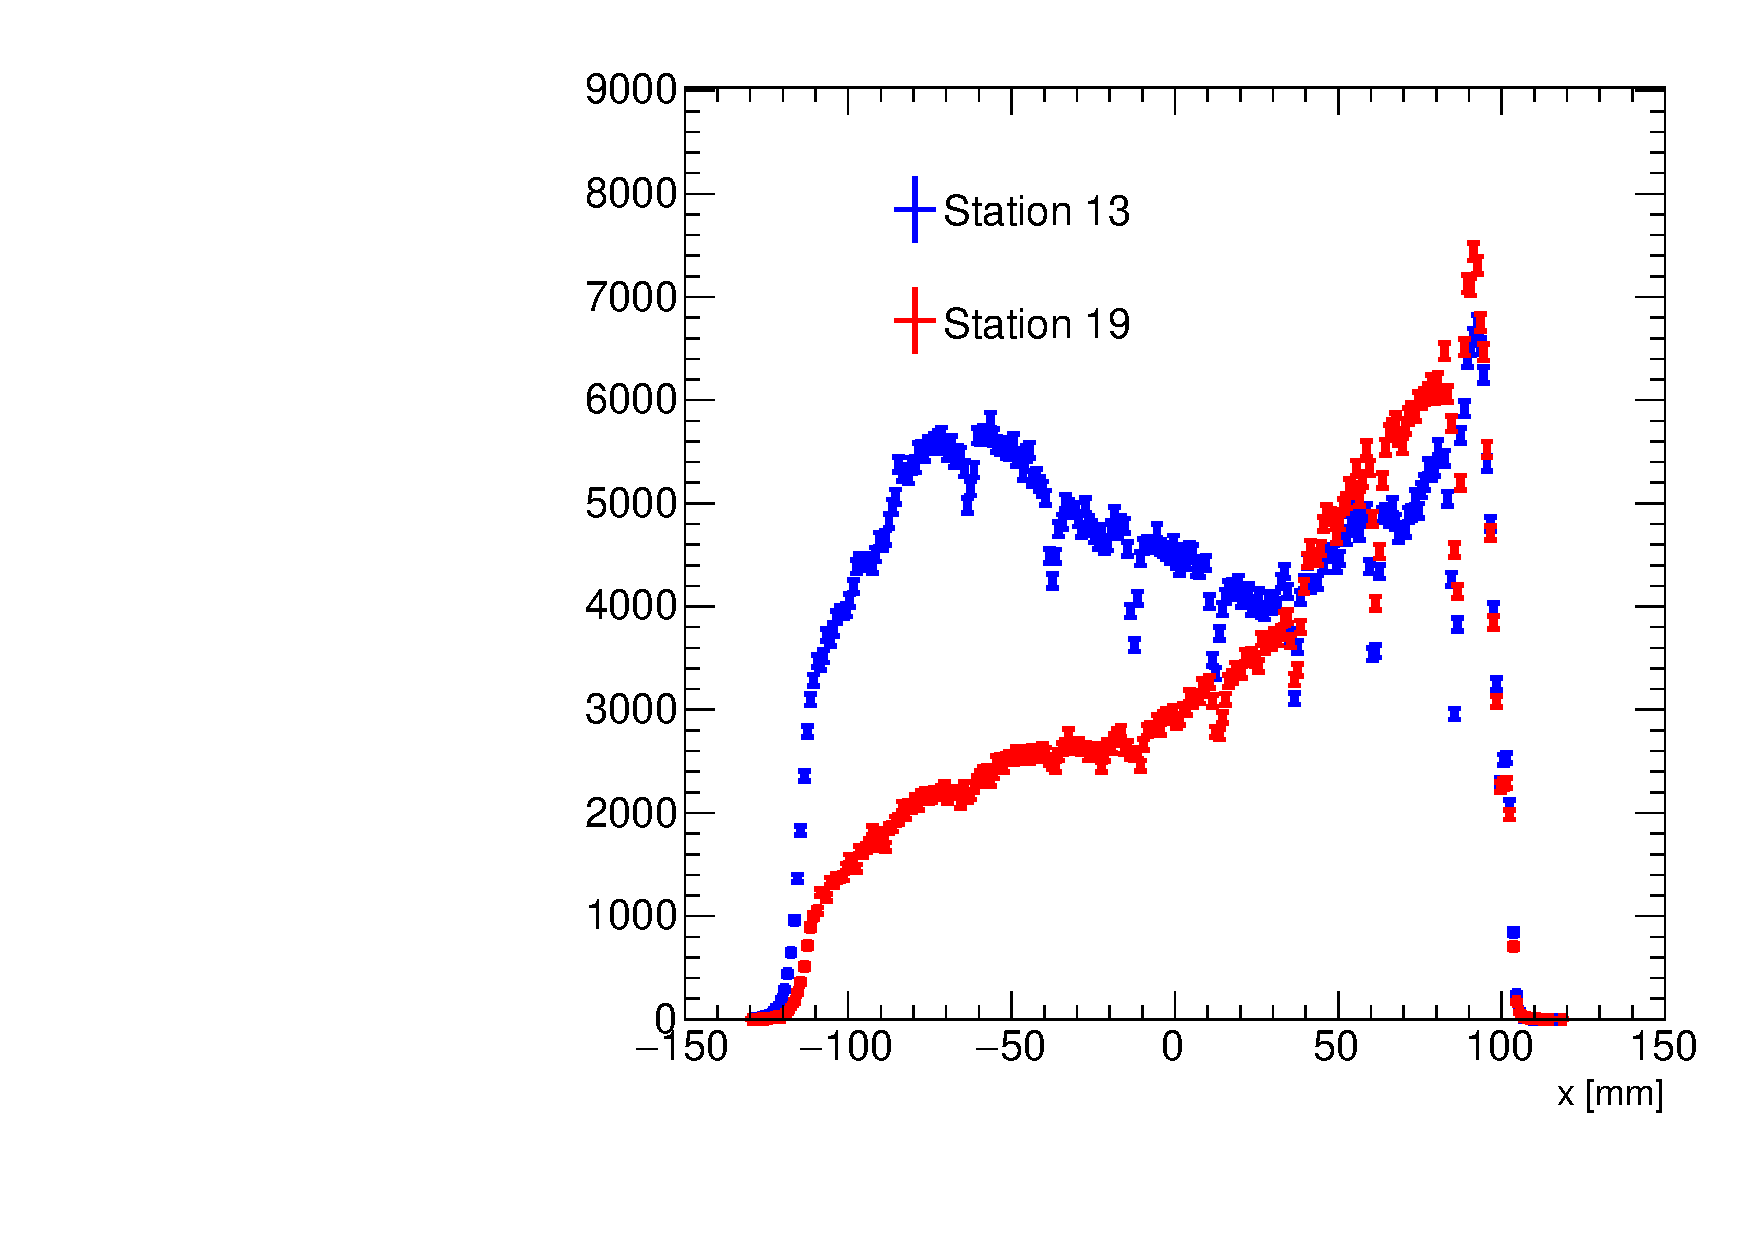
\includegraphics[width=0.4\textwidth]{figures/St13_mu_x.pdf}
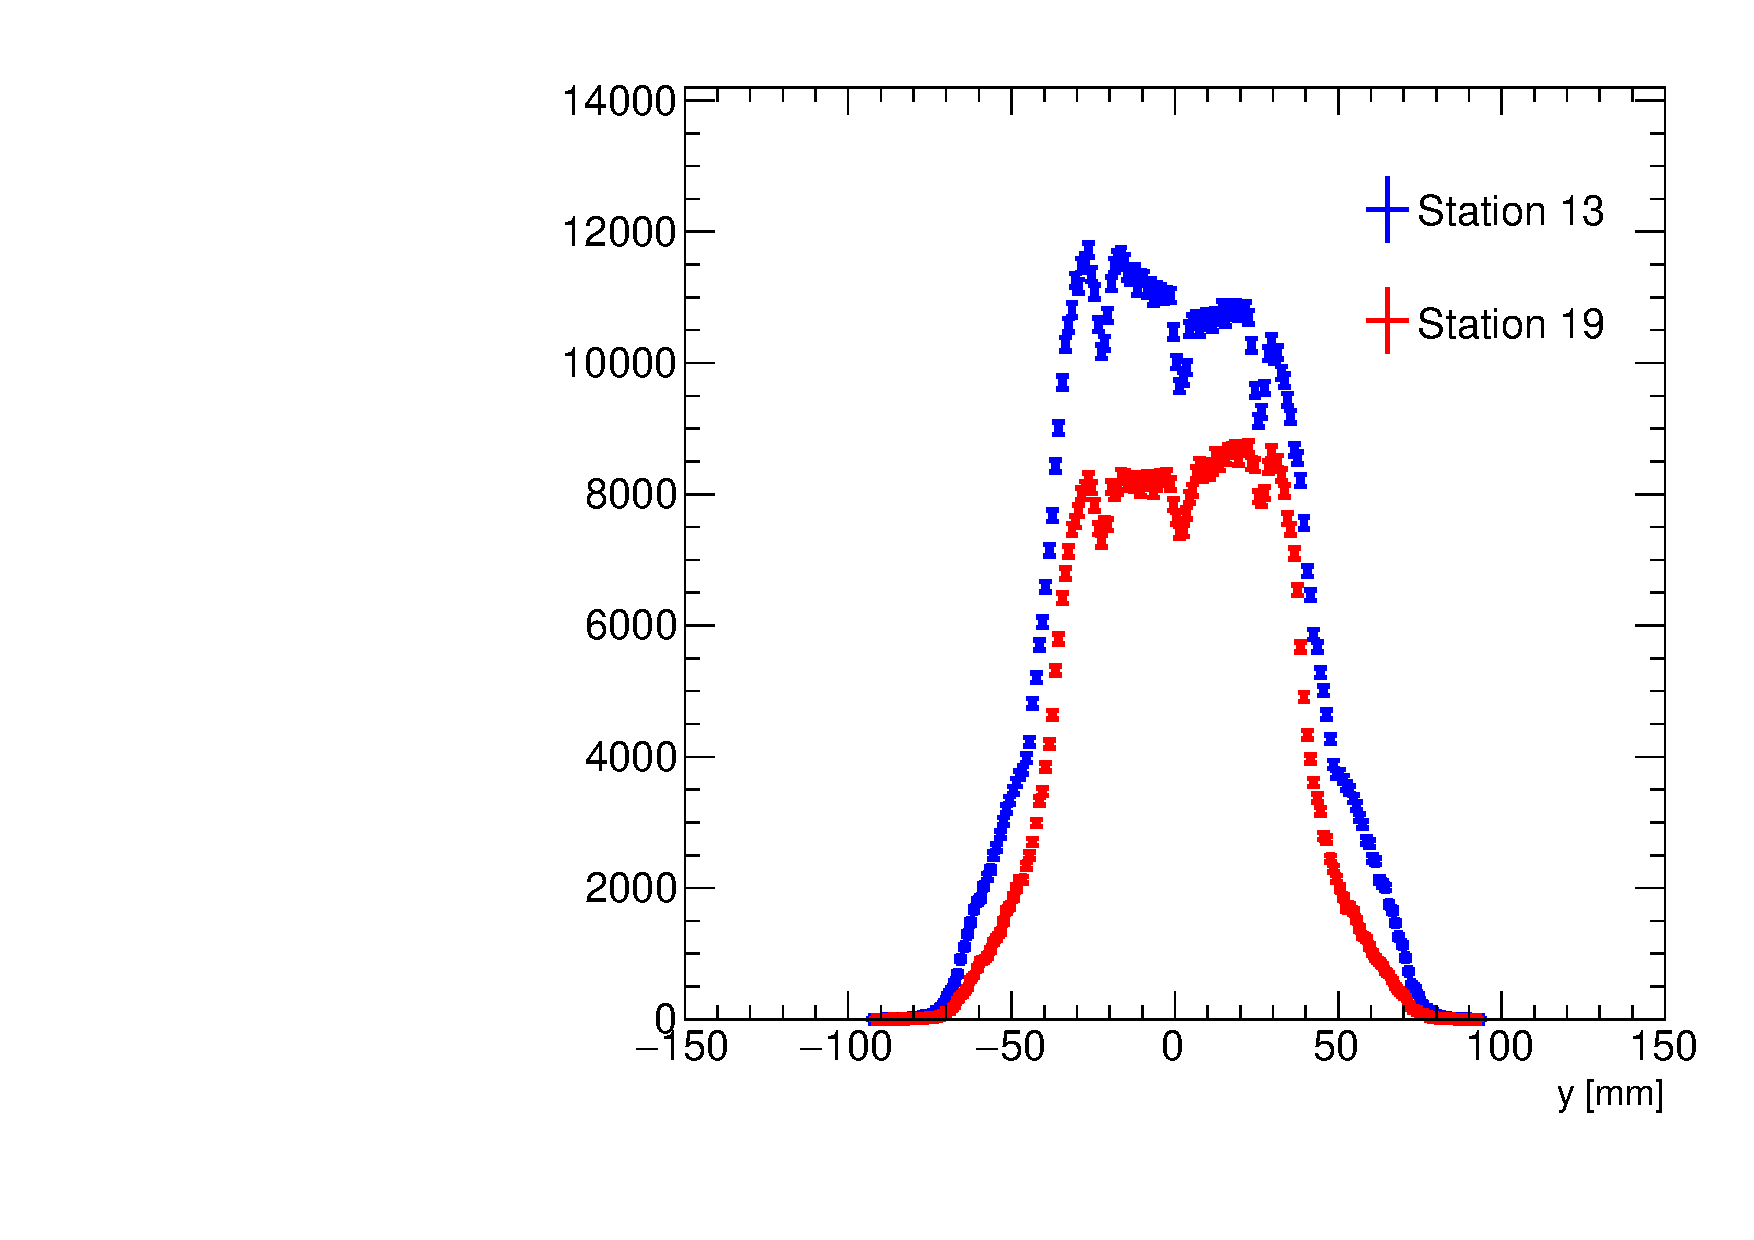
\includegraphics[width=0.4\textwidth]{figures/St13_mu_y.pdf}
\caption{Muon track x (left) and y (right) positions at Station 13 and 19 calorimeters. \label{fig:muon_posn}}
\end{figure}

The x and y distributions for muon tracks extrapolated to calorimeter face are shown in Fig.~\ref{fig:muon_posn}. Comparing the x distributions with those obtained from the calorimeter-only analysis, the muons in Station 13 appear to contain a roughly equal mix of ``first calorimeter in a triple'' (peaked to the right) and ``third calorimeter (peaked to the left). In Station 19, the distribution is consistent with a larger population of ``first calorimeter in a triple''. This trend is consistent with the higher number if muons observed in calorimeters 10, 11 and 12, and the lower number observed in 16,17 and 18 (Figure 3).

\begin{figure}[h]
\centering
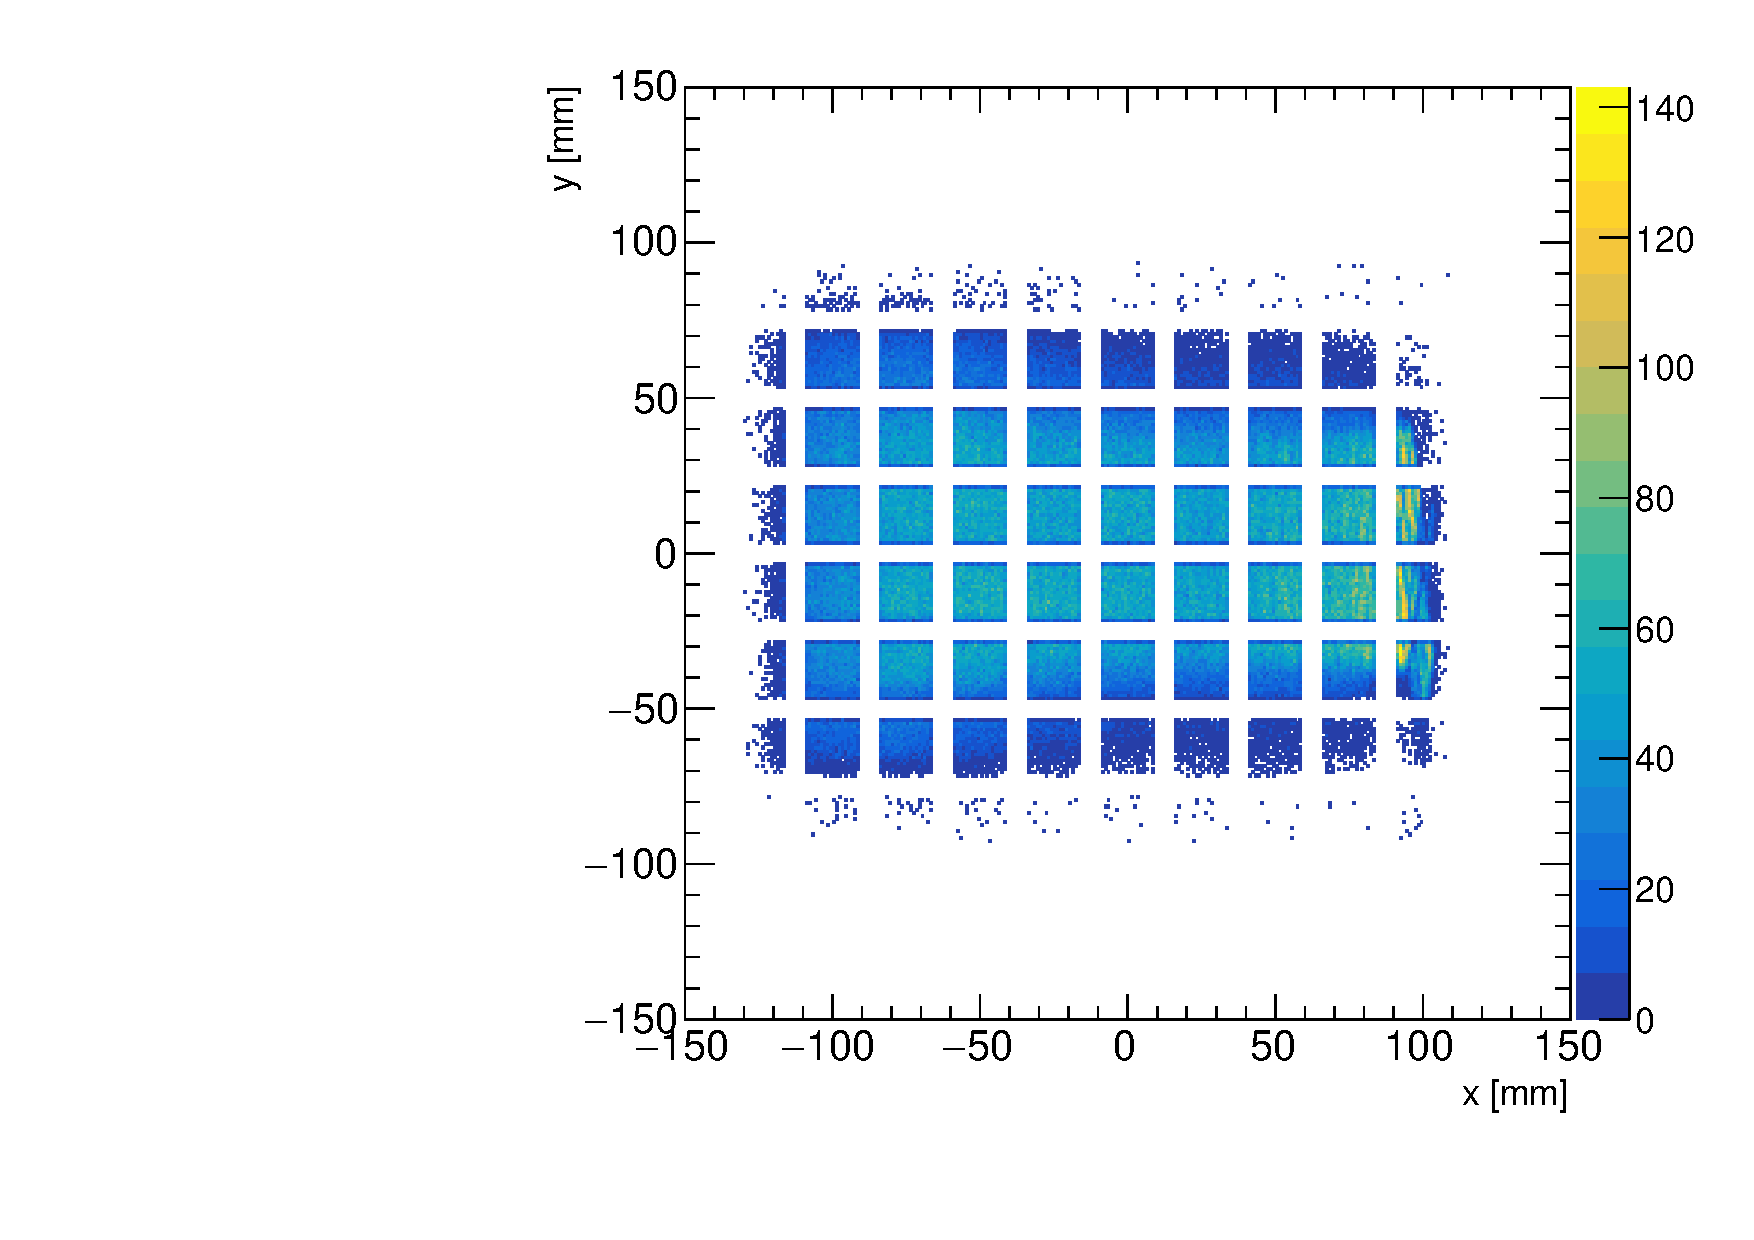
\includegraphics[width=0.4\textwidth]{figures/St13_mu_xy_fid.pdf}
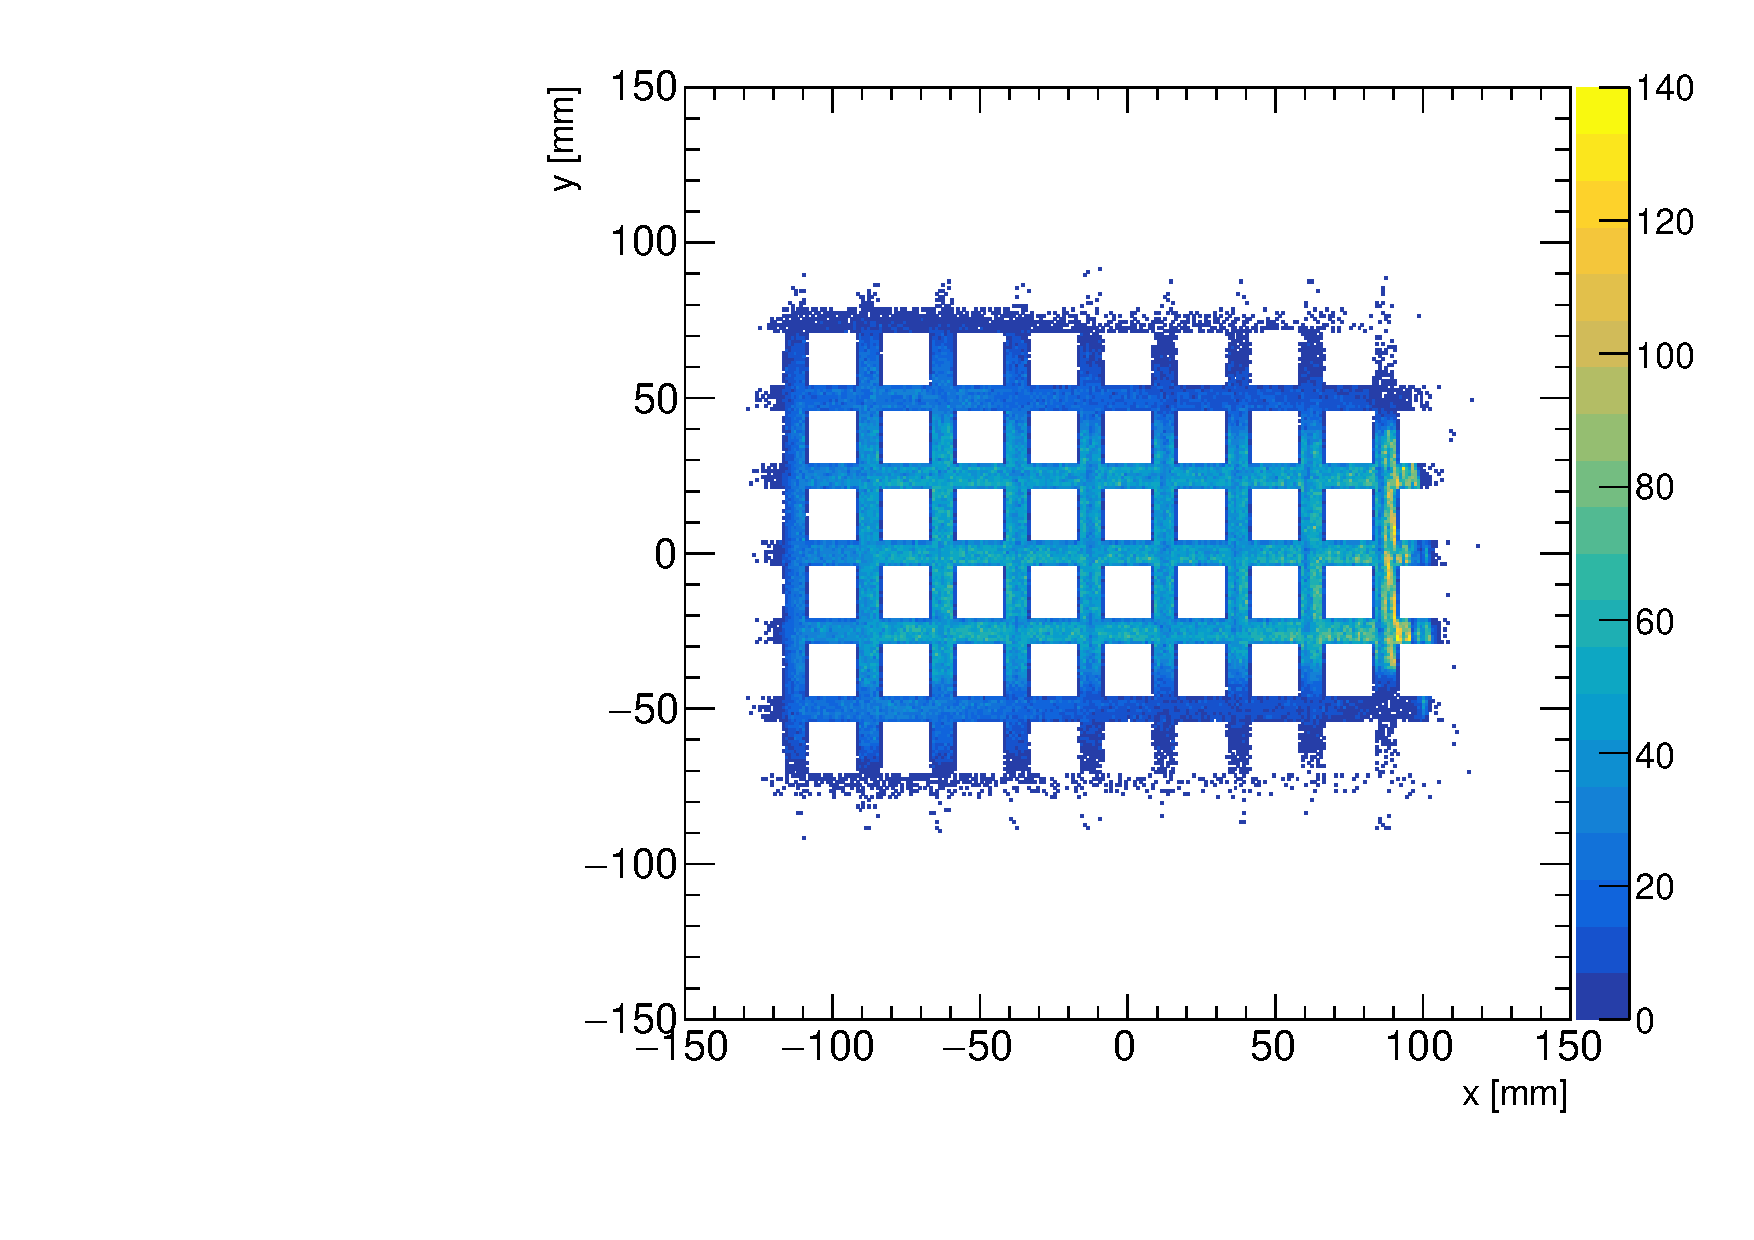
\includegraphics[width=0.4\textwidth]{figures/St13_mu_xy_nfid.pdf}
\caption{Extrapolated track positions for ``fiducial'' (left) and ``non-fiducial'' muons, in Station 13.\label{fig:fiducial}}
\end{figure}

\begin{figure}[h]
\centering
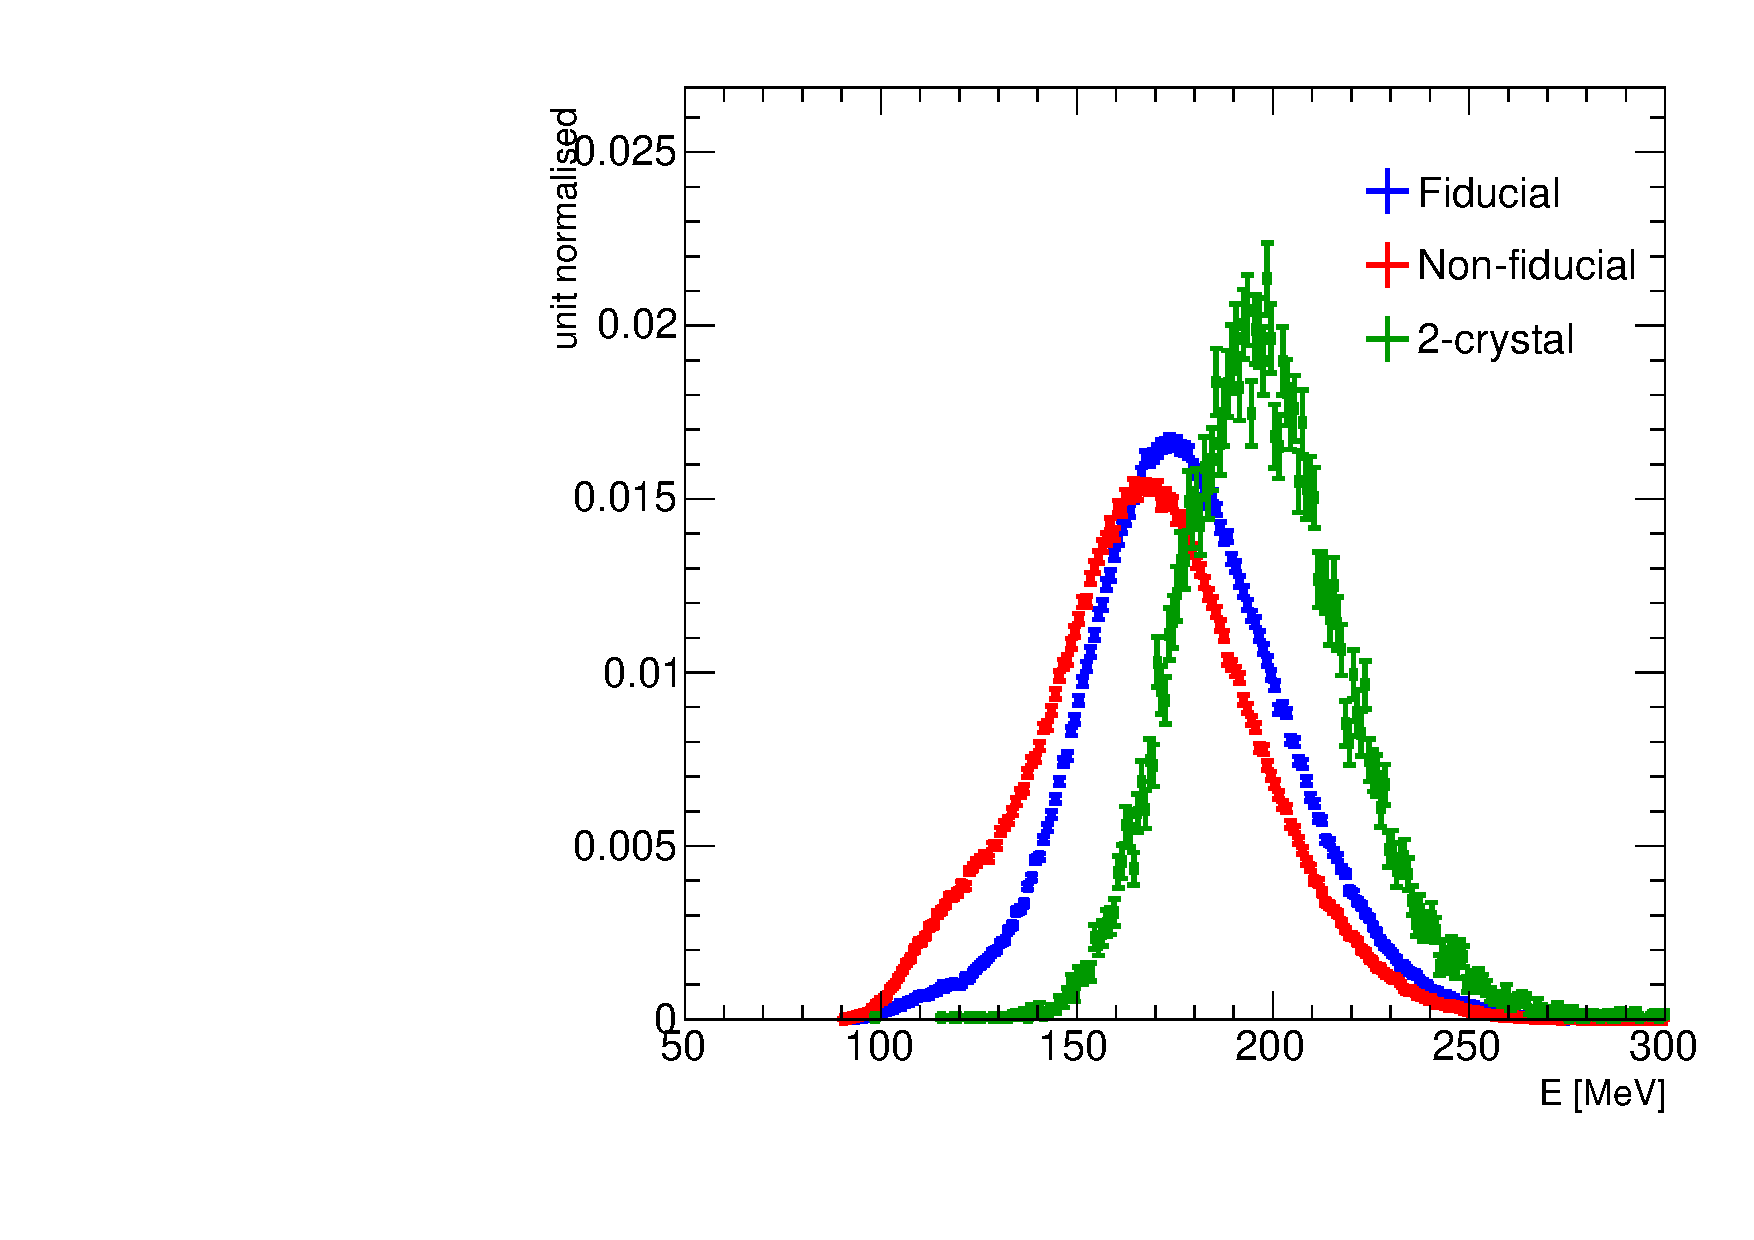
\includegraphics[width=0.4\textwidth]{figures/St13_mu_E_fid.pdf}
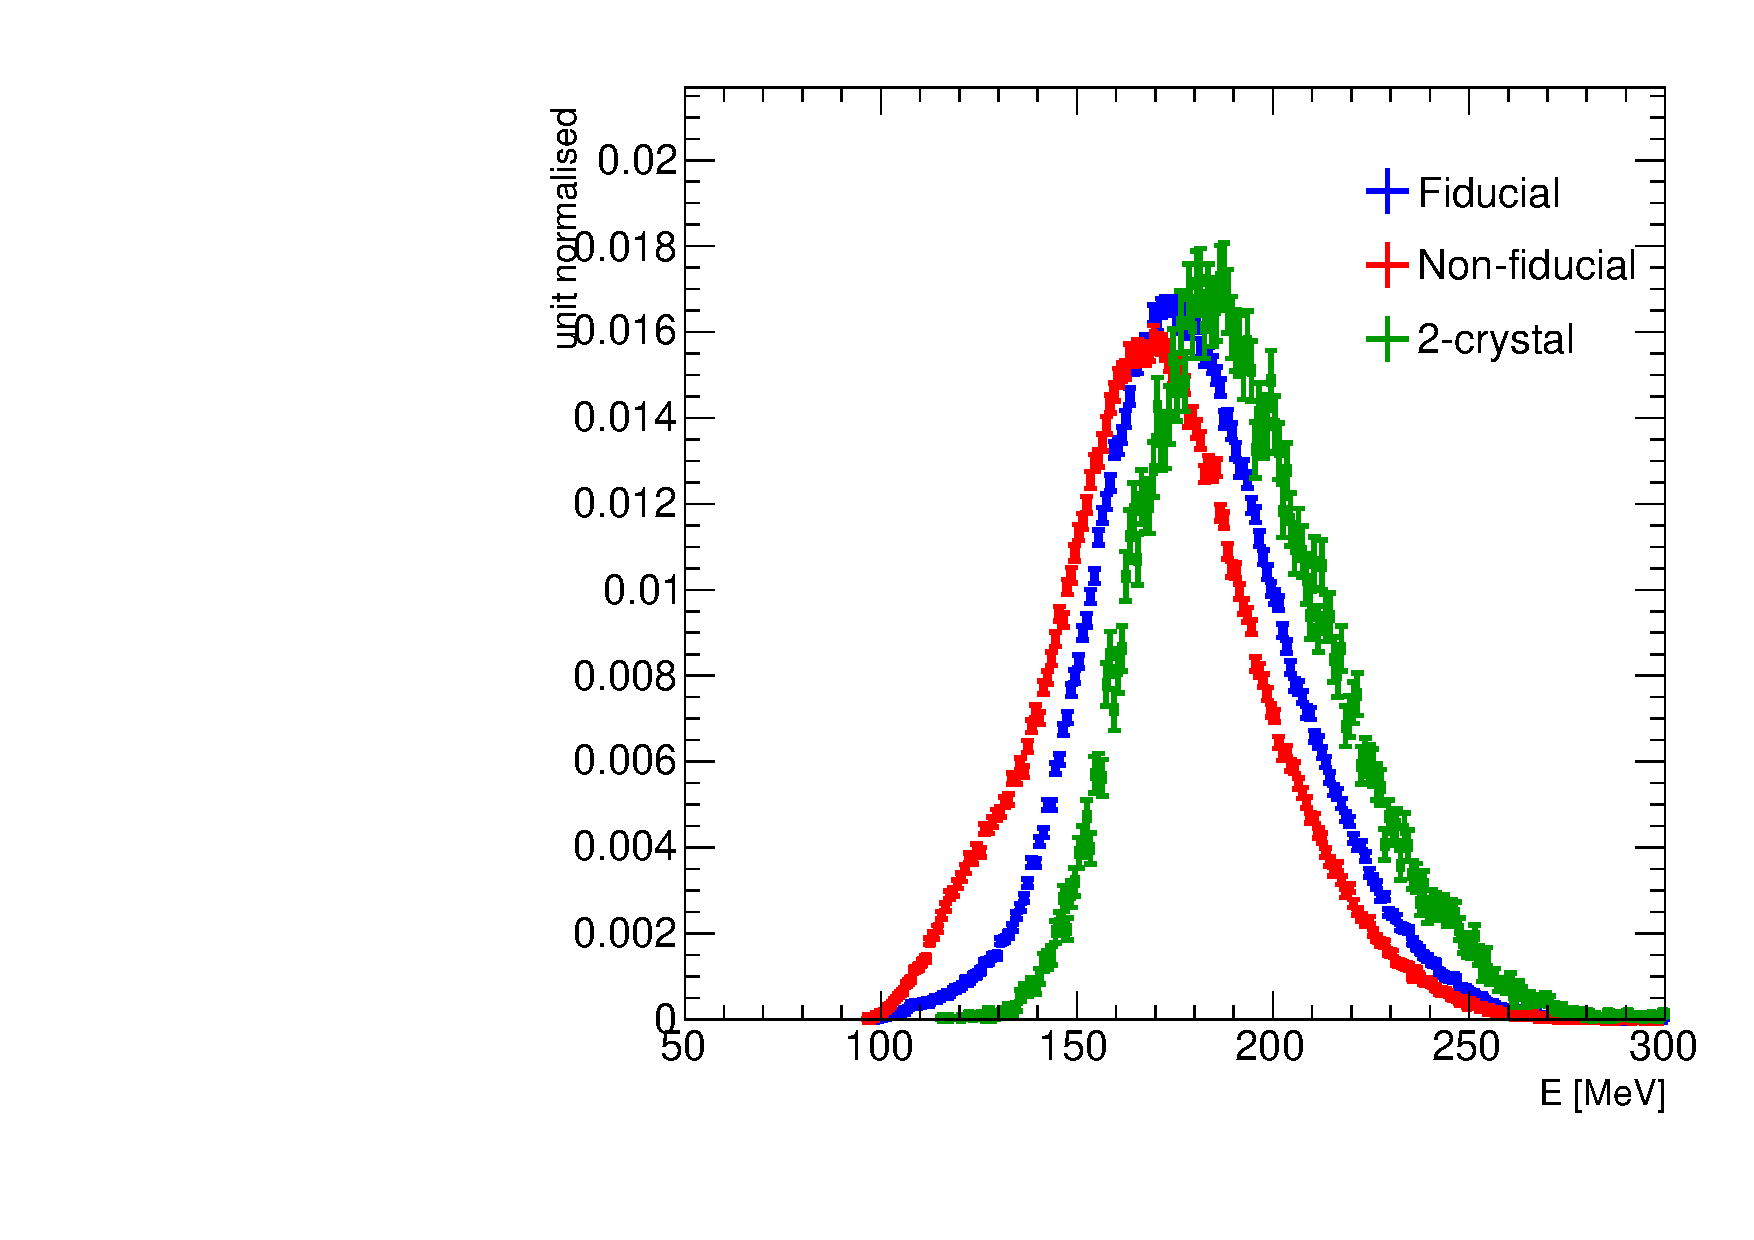
\includegraphics[width=0.4\textwidth]{figures/St19_mu_E_fid.pdf}
\caption{Muon energy distributions in Station 13 (left) and 19 (right) calorimeters. \label{fig:E_dep}}
\end{figure}

Finally, the tracker-based muon sample was to identify any dependence of the reconstructed calorimeter energy on the position and kinematics of the muon track. The energy of the calorimeter cluster shows only minimal dependence on the angle of the incoming muon track, but a strong dependence is visible when the path of the muon crosses a crystal boundary. To study this, each crystal is divided into equal-area ``fiducial'' and ``non-fiducial'' regions, with fiducial being defined as the central 17.7 mm in both x and y. The positions of extrapolated tracks hitting fiducial and non-fiducial regions is shown in Fig.~\ref{fig:fiducial}. The matched calorimeter cluster energy is show in Fig.~\ref{fig:E_dep} for three cases: single-crystal clusters in fiducial regions; single-crystal clusters in non-fiducial regions; and any cluster containing more than one crystal. Non-fiducial muons peak at a lower energy, consistent with some energy lost either crossing a crystal boundary or when a second crystal is below threshold. The two-crystal clusters are higher in both stations, though significantly more so in Station 13. This may relate to the backgrounds discussed in Section 4.1, but is not expected to have any impact on the L(t) function.



\end{document}


